\documentclass[fleqn,xcolor={usenames,dvipsnames}]{beamer}
\usepackage{amsmath} % {amssymb,amsfonts}
% \usepackage{colortbl}

% \usepackage{booktabs, multicol, multirow, adjustbox}
\usepackage{array, adjustbox,url}
\usepackage{pifont,marvosym} % wasysym

\usepackage{multimedia}
\usepackage[normalem]{ulem}
\usepackage{framed,color,ragged2e}
\usepackage[absolute,overlay]{textpos}
\definecolor{shadecolor}{rgb}{0.8,0.8,0.8}
\usetheme{boxes}
\setbeamertemplate{navigation symbols}{}
\usepackage{xcolor}
\usepackage{tikz}
\usetikzlibrary{shapes,arrows}
\usetikzlibrary{positioning}
\usetikzlibrary{calc}
% \usetikzlibrary{cd}

\newcolumntype{R}[2]{%
    >{\adjustbox{angle=#1,lap=\width-(#2)}\bgroup}%
    l%
    <{\egroup}%
}
\newcommand*\rot{\multicolumn{1}{R{45}{1em}}}% no optional argument here, please!


\title{Asynchronous messaging strategy}
\subtitle{Axolotl-style long-term forward secrecy for a Sphinx mixnet}
% Now we have to build a GNU one!

\author[Burdges]{Jeff Burdges}
\institute{
  
\includegraphics[scale=0.2]{../logos/gnunet-logo.pdf}

  \vfill
  
\includegraphics[scale=0.2]{../logos/inria.pdf}
}
\date{28.6.2015}


\begin{document}


{\setbeamertemplate{footline}{}
\begin{frame}
\titlepage
\end{frame}
}
\setcounter{framenumber}{0}


% Discuss OtR?
% Axolotl
% .. with side keys
% Sphinx
% ... SURBs
% Messaging
% Xolotl


\begin{frame}{E-mail: Asynchronous messaging}
  \begin{itemize}
  \item Email with GnuPG provides authenticity and confidentiality... % \pause
  \item ... but fails to protect meta-data
  \item ... and also fails to provide {\em forward secrecy} aka {\em key erasure}
  \end{itemize}
\end{frame}


\begin{frame}{Why forward secrecy?}
Imagine Eve records
 your GnuPG encrypted emails {\it now}, say here:
% like say in Blufdale Utah.

\medskip
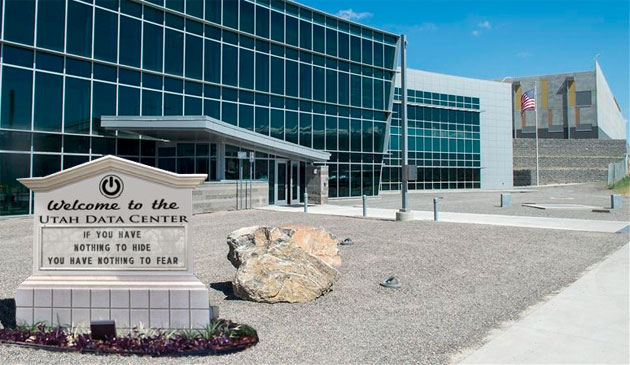
\includegraphics[width=\textwidth]{../pics/nsa-utah-data-center-entrance.jpg}
\medskip

If Eve {\it ever} compromises your private key in the {\it future},
then she can read the encrypted emails you sent {\it today}.
\end{frame}


\begin{frame}{Synchronous messaging}
 \begin{columns}[T]
 \column{0.48\textwidth}
 \smallskip
%  State of the art:
  \begin{center}
    {\bf XMPP/OtR over Tor}
  \end{center}
  \begin{itemize}
  \item Forward secrecy from OtR
  \item User-friendly key exchange
  \item Location protection (Tor)
  \item ... but not asynchronous
  \item ... and leaks meta-data % to server
  \item No encrypted file transfers
  \end{itemize}

%  \begin{center}
%    {\bf TextSecure}
%  \end{center}

\column{0.52\textwidth}
\includegraphics[page=2,scale=0.4,trim=70 0 0 20, clip]{../pics/nsa_v_otr}
\end{columns}
\end{frame}


%\begin{frame}{Key erasure aka Forward secrecy}
\begin{frame}{Why is OtR synchronous only?}%{Background: OTR}

{\small
We achieve {\em forward secrecy} through {\em key erasure} by negotiating 
an ephemeral session key using Diffie-Hellman.  

\medskip
Diffie-Hellman key exchange uses commutativity of exponentiation:
$$ A^b = (g^a)^b = (g^b)^a = B^a \bmod p $$
Elliptic curve Diffie-Hellman uses commutativity of scalar multiplication:
$$ d_A Q_B = d_A d_B G = d_B d_A G = d_B Q_A $$}
  \begin{figure}[th]
    \begin{minipage}[b]{0.45\linewidth}
      \begin{center}
	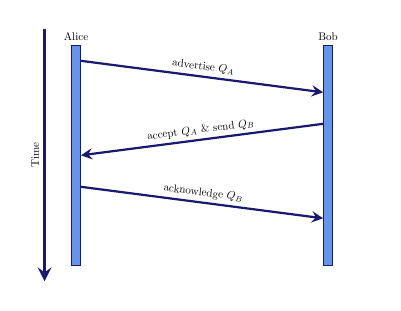
\begin{tikzpicture}[scale = 0.4,
            transform shape,
            msglabel/.style    = { text = Black, yshift = .3cm,
                                   sloped, midway },
            okmsg/.style       = { ->, color = MidnightBlue, thick,
                                   >=stealth },
            rstmsg/.style      = { ->, color = BrickRed, thick,
                                   >=stealth }
	  ]
	  \node[draw = MidnightBlue,
	    fill = CornflowerBlue,
	    minimum width = .3cm,
	    minimum height = 7cm
	  ] (h1) at (-4, 0) {};
	  \node[draw = MidnightBlue,
	    fill = CornflowerBlue,
	    minimum width = .3cm,
	    minimum height = 7cm
	  ] (h2) at (4, 0) {};
	  \node[above = 0cm of h1] {Alice};
	  \node[above = 0cm of h2] {Bob};

	  \path[->, color = MidnightBlue, very thick, >=stealth]
	    (-5, 4) edge
	    node[rotate=90, text = Black, yshift = .3cm] {Time}
	    (-5, -4);
	  \path[->, color = MidnightBlue, thick, >=stealth]
	    ($(h1.east)+(0,3)$) edge
	    node[text = Black, yshift = .3cm, sloped] {advertise $Q_A$}
	    ($(h2.west)+(0,2)$);
	  \path[->, color = MidnightBlue, thick, >=stealth]
	    ($(h2.west)+(0,1)$) edge
	    node[text = Black, yshift = .3cm, sloped] {accept $Q_A$ \& send $Q_B$}
	    ($(h1.east)+(0,0)$);
	  \path[->, color = MidnightBlue, thick, >=stealth]
	    ($(h1.east)+(0, -1)$) edge
	    node[text = Black, yshift = .3cm, sloped] {acknowledge $Q_B$}
	    ($(h2.west)+(0, -2)$);
	  \node at (5.3, 0) {};
	\end{tikzpicture}
      \end{center}
    \end{minipage}
    \hspace{0.5cm}
    \begin{minipage}[b]{0.45\linewidth}
      \small
      Private keys: \\
      \hspace*{2pt} $d_A$, $d_B$ \\
      \smallskip

      Public keys: \\
      \hspace*{2pt} $Q_A = d_A G$ \\
      \hspace*{2pt} $Q_B = d_B G$ \\
      \bigskip
    \end{minipage}
  \end{figure} % \pause

\pause

Answer: 
All three messages of the Diffie-Hellman key exchange must complete 
before OtR can use a new ratchet key.
\end{frame}


% \begin{frame}{Why is OtR synchronous only?}%{Background: OTR}
% Answer 1:
% All three messages of the Diffie-Hellman key exchange must complete 
% before OtR can use a new ratchet key.
%
% \bigskip\bigskip
%
% Answer 2:
% OtR overlays on traditional instant messaging protocols, 
% like XMPP, which all use named accounts on designated servers.
% So two OtR sessions might originate from different devices.
% \end{frame}


\begin{frame}{Axolotl by Trevor Perrin and Moxie Marlenspike}
\begin{columns}[T]
\column{0.55\textwidth}
% Mexican walking fish
% salamander 
% gills resemble trees
% related to tiger salamander 
% neoteny metamorposis into similar salimander if given enough iodine or hormones 

Idea from Silence Circle's SCIMP: \\
\hspace*{2pt} Replace our key with its own hash.

\medskip

Good: New key in zero round trips.

\smallskip

Bad: Stays compromised in future.

\bigskip

Approach: \\
\hspace*{2pt} Run DH whenever possible \\
\hspace*{2pt} Iterate key by hashing otherwise 

% 

\column{0.45\textwidth}
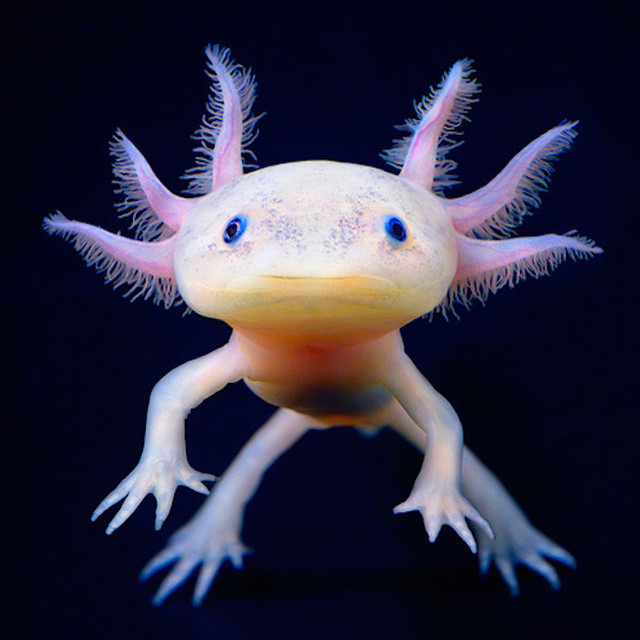
\includegraphics[width=\textwidth]{../pics/axolotl_animal-1.jpg}
\end{columns}

\medskip

\begin{quote}
``[Axolotl] combines the .. forward secrecy [of] a hash iteration ratchet like SCIMP [with the] future secrecy .. of a DH ratchet like OtR'' % \\
\hfill --- Moxie Marlenspike % (TextSecure)
\end{quote}
\end{frame}


\begin{frame}{Axolotl by Trevor Perrin and Moxie Marlenspike}
\begin{columns}[T]
\column{0.6\textwidth}
Approach: \\
\hspace*{2pt} Run DH whenever possible \\
\hspace*{2pt} Iterate key by hashing otherwise 

\medskip
Way less boo keeping! \\
\smallskip
Header is one DH public key, \\
 \hspace*{2pt} which one can encrypt.

\onslide<2>{
\bigskip
TripleDH provides authentication \\
 \hspace*{2pt} with deniability,  although a \\ 
 \hspace*{2pt} ratchet cannot be fully anonymous. 
%}

%\onslide<3>{
\bigskip
Neutral against Shor's algorithm \\
 \hspace*{2pt} running on a quantum computer. \\
}

\column{0.4\textwidth}
\includegraphics[width=\textwidth]{../pics/axolotl_diagram}
% \vspace*{-20pt}
% \includegraphics[width=0.95\textwidth,trim={0 0 0 47},clip]{axolotl_diagram}
\end{columns}
\end{frame}


% \begin{frame}{Axolotl vs. Anonymity}
% \end{frame}


\begin{frame}{Axolotl with side-keys}
\begin{columns}[T]
\column{0.6\textwidth}
Alice/Bob keeps resending the same key 
% since message can be lost
\begin{center}
Can we do better?
\end{center}

\onslide<2>{
Keep two associative arrays: \\
\begin{itemize}
\item RecievingKeys -
 Keys we proposed and hold until our contact uses. % \\
% \hspace*{6pt}  (symmetric or private) 
\item SendingKeys - 
 Keys we received and shall attempt to use. % \\
% \hspace*{6pt}  (symmetric or public)
\end{itemize}

\bigskip
Two rules:
\begin{enumerate}
\item Sidekey usage much be announced
\item Sidekeys bind permanently to \\
 one individual ratchet DH keys
\end{enumerate}
}

\column{0.4\textwidth}
\includegraphics[width=\textwidth]{../pics/axolotl_diagram}
% \vspace*{-20pt}
% \includegraphics[width=0.95\textwidth,trim={0 0 0 47},clip]{axolotl_diagram}
\end{columns}
\end{frame}


\begin{frame}{Axolotl with {\em symmetric} side-keys}
\begin{columns}[T]
\column{0.6\textwidth}
Axolotl headers should be encrypted, \\
\hspace*{2pt} using a previous ratchet state, \\
\hspace*{2pt} which must be announced.

\medskip
If our sidekey is symmetric, then simply replace that previous ratchet state.

\bigskip
Applications:
\begin{itemize}
\item Conferences, couriers, etc.
\item Rogaway's Bigkeys
\item Socialist Millionaires' protocol?
\item Mixnets?
\end{itemize}

\column{0.4\textwidth}
\includegraphics[width=\textwidth]{../pics/axolotl_diagram}
% \vspace*{-20pt}
% \includegraphics[width=0.95\textwidth,trim={0 0 0 47},clip]{axolotl_diagram}
\end{columns}
\end{frame}

\begin{frame}{Axolotl with {\em asymmetric} side-keys}
\begin{columns}[T]
\column{0.6\textwidth}
If our sidekey is a public key, then  \\
\hspace*{2pt} send an encrypted update $u$ to \\
\hspace*{2pt} the rootkey in the message itself. % \\
$$r \mapsto H(u,r)$$

Apply this update after the DH update.
% \hspace*{2pt} because the receiver needs the new chain key.

By Rule 2, repeat $u$ exactly throughout\\
\hspace*{2pt} the ratchet DH key's lifetime. \\
And only apply it once on each side.

\bigskip
Applications:
\begin{itemize}
\item Apply post-quantum lazily 
\item Big ass public keys
\item Algorithm diversity
\end{itemize}

\column{0.4\textwidth}
\includegraphics[width=\textwidth]{../pics/axolotl_diagram}
% \vspace*{-20pt}
% \includegraphics[width=0.95\textwidth,trim={0 0 0 47},clip]{axolotl_diagram}
\end{columns}
\end{frame}


%%% Sphinx mixnet


\begin{frame}{Sphinx mixnet by George Danezis and Ian Goldberg}
\begin{center}

\includegraphics[width=0.8\textwidth]{../pics/Sphinx}

Mixnets use cryptography in mysterious ways
\end{center}
\end{frame}


\begin{frame}{Sphinx mixnet by George Danezis and Ian Goldberg}
Provably secure in the universal composability model \\
\hspace*{2pt} [Camenisch \& Lysyanskaya '05, Canetti '01]
\begin{enumerate}
\item Provides correct onion routing
\item Integrity, meaning immunity to long-path attacks
\item Security, including \\
\hspace*{2pt} wrap-resistance{\small $^*$} and \\
\hspace*{2pt} indistinguishability of forward and reply messages
\item[] Replay protection implemented by Bloom filter
\end{enumerate}

\bigskip
\bigskip
\bigskip

{\small $^*$ Wrap-resistance helps prevent nodes from acting as decryption oracle.}
\end{frame}


\begin{frame}{Sphinx by George Danezis and Ian Goldberg}
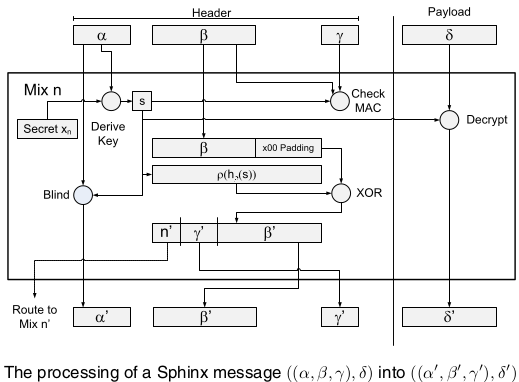
\includegraphics[width=\textwidth]{../pics/Sphinx-diagram}
\end{frame}
% LIONNESS???


\begin{frame}[t]{Replies in Sphinx}
Can a recipient be anonymous? \\
Yes!  With a Single-Use Reply Block (SURB).

\medskip
An anonymous recipient must
\begin{itemize}
\item create the Sphinx header $(\alpha, \beta, \gamma)$, 
\item communicate it to the sender $n$ in advance, and 
\item remember symmetric keys since $\delta$ gets encrypted at each hop.
\end{itemize}

\bigskip
\bigskip
\pause
All keys are ephemeral in Sphinx to enable replay protection, \\
\hspace*{2pt} so SURBs have a limited lifetime.

\end{frame}


\begin{frame}{Bi-directional anonymity in Sphinx}
Can both parties be anonymous? \\
Yes!  With a cross-over point that violates wrap-resistance.

\medskip
We modify the protocol:
\begin{itemize}
\item Reserve twice the space for the Sphinx header. 
\item Onion encrypt and HMAC the extra space with the header.{\small $^*$}
\item Add a method to replace a header with this extra space. 
 and generate its extra space filler deterministically from a seed $s$. 
\end{itemize}
Now a SURB consists of \\
\hspace*{2pt} a starting node $n$, \ the seed $s$, \ and \\
\hspace*{2pt} our Sphinx header $(\alpha, \beta, \gamma)$ valid from $n$.

\medskip
Use this SURB by building a Sphinx header to $n$ that \\
\hspace*{2pt} onion decrypts itself to $s$ and its extra space  to $(\alpha, \beta, \gamma)$.

\bigskip\bigskip

{\small $^*$ We onion encrypt the Sphinx headers backwards, including those that use SURBs,
but the SURB itself must encrypt this extra space forwards.}

\end{frame}


\begin{frame}{Tiered delivery strategies}
% Synchronous 
Quick replies :
If users share SURBs with one another, then \\ % {\small $^1$}
\hspace*{2pt} they send messages directly but only during one mixnet session.

\medskip

Mailbox accounts for asynchronous messages : 
\begin{itemize}
\item Created on a random mixnet relay $n$, \\
 \hspace*{2pt} assigned a mailbox id $m$ and a shared secret $k$.
\item Checked by supplying with quick reply SURBs
\end{itemize}

\medskip
\pause

Frequent contacts : Give SURBs for sending to primary mailbox %{\small $^2$}

\medskip

Infrequent or public contact options : 
\begin{itemize}
\item Give real delivery details for a secondary mail server
\item Could require tokens or group signatures, or proof-of-work
\item Form a tree of secondary mailboxes
\end{itemize}

% {\small $^1$ We could go even faster using HORNET-like circuits.}
% {\small $^2$ Add a short segment encrypted to communicate the identity of the SURB used to reach the mailbox }

\end{frame}

\begin{frame}[t]{Ratchet for Sphinx }
\begin{columns}[T]
\column{0.60\textwidth}

Can we integrate a ratchet with Sphinx?

\medskip
Axolotl won't work because : 
\begin{itemize}
\item Relays never message users
\item Cannot reuse curve elements
\end{itemize}

\medskip
Ideas : 
\begin{itemize}
\item Relays share new keys with the whole network for replay protection \\
% \hspace*{2pt} Key lifetime = SURB lifetime
\item Users should learn what messages made it eventually
\end{itemize}

\column{0.40\textwidth}
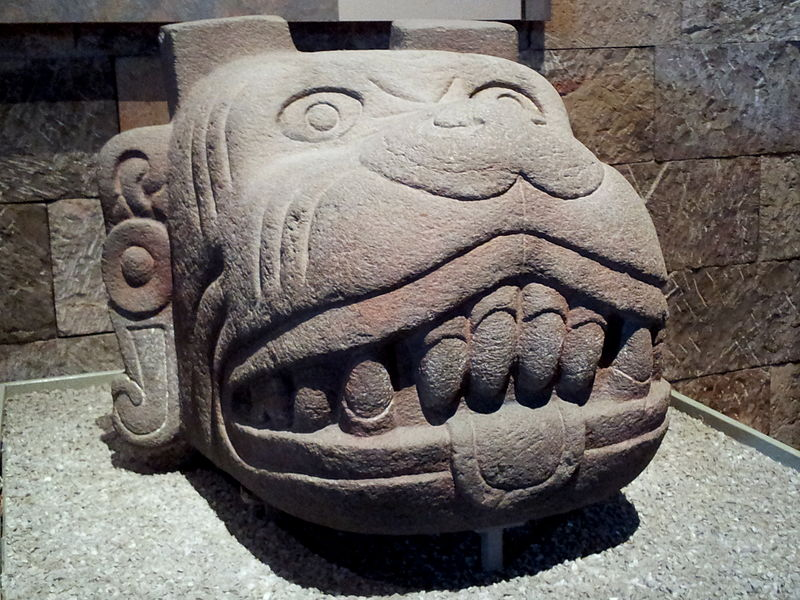
\includegraphics[width=1.35\textwidth,trim={80 0 0 0},clip]{../pics/Xolotl_muz}
\begin{center}
Xolotl \\
Sphinx + Axolotl
\end{center}
\end{columns}

\end{frame}


\begin{frame}[t]{Relay key replacement }
Replay protection requires that relays replace keys regularly. 
\begin{columns}[T]
\column{0.6\textwidth}
{\hfil Key lifetime = SURB lifetime \hfil}

\medskip
Longer lifetime improves:
\begin{itemize}
\item Delivery convenience
\end{itemize}

\smallskip
Shorter lifetime improves:
\begin{itemize}
\item Throughput 
\item Memory footprint
\item Forward-secrecy
\end{itemize}

\column{0.4\textwidth}
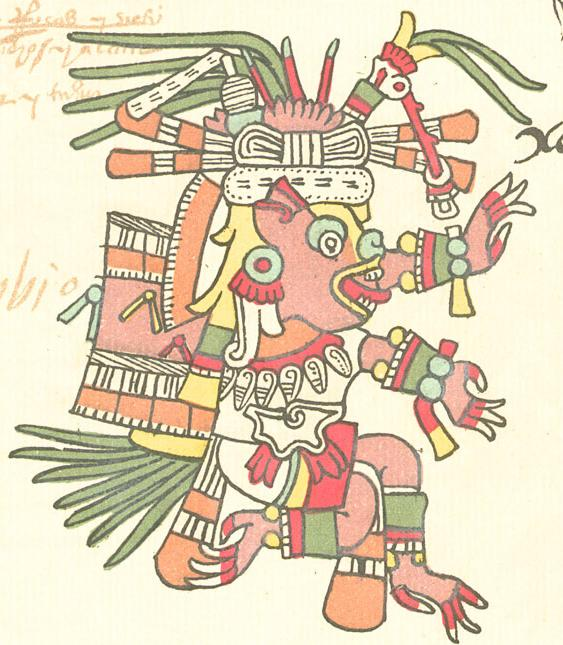
\includegraphics[width=1.2\textwidth]{../pics/Xolotl}
\end{columns}
\end{frame}


\begin{frame}[t]{Acknowledging ratchet state }
\begin{columns}[T]
\column{0.5\textwidth}
Idea: Client directs ratchet state

\bigskip
Chain keys evolve like Axolotl, 
 \hspace*{2pt} producing leaf keys. % \\ not message keys.

\smallskip
Create message keys by hashing \\
 \hspace*{2pt} a leaf key with a Sphinx ECDH \\ % result.

\smallskip
 \hspace*{10pt} $\textrm{mk} = H(\textrm{lk},H'(\textrm{ECDH}(\textrm{u},\textrm{r})))$

\medskip
\onslide<2>{
Packets identify the message key from which their chain started.

\smallskip % \hspace*{2pt}
And their leaf key sequence no. % number.
%}

\smallskip
% \onslide<3>{ % \hspace*{2pt}
And parent max sequence no.
%And their parent chain's max sequence no.
}

\column{0.5\textwidth}
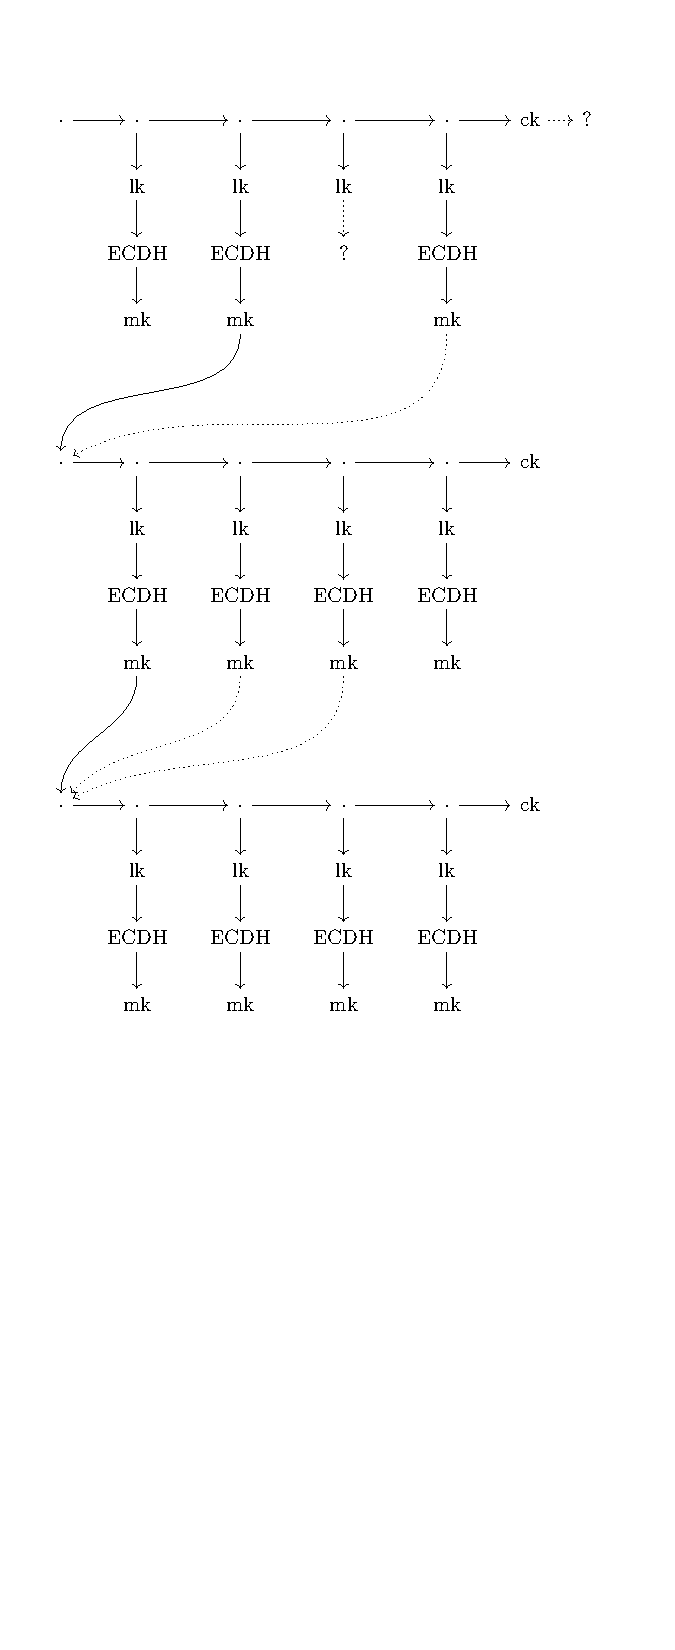
\includegraphics[width=0.95\textwidth,trim={0 0 0 47},clip]{Xolotl_diagram0}
\end{columns}
\end{frame}



\begin{frame}{Wait. Aren't ratchets only pseudononymous? }

We cannot use the Xolotl ratchet for every mixnet hop, but \\
the ratchet should be suitable for certian situations.

\bigskip

Guard nodes can use a session ratchet initialized with:
\begin{itemize}
\item post-quantum key exchange, or 
\item another longer term ratchet, maybe.
\end{itemize}

\bigskip

Third hop out of a five hope circut: \\
\begin{itemize}
\item Long-term ratchet is okay, but only pseudonymous
\item Initializing from a longer term ratchet is okay
\end{itemize}

\bigskip
Other hops require greater care

\[ \textrm{User} \to \textrm{Guard} \to \textrm{Anon} \to \textrm{Pseudo} \to \textrm{Anon} \to \textrm{Cross} \to \cdots \]

\end{frame}




\end{document}












\begin{frame}
\end{frame}


\begin{frame}
\end{frame}


\begin{frame}
\end{frame}



























\begin{frame}{Brian Warner's Delivery Properties}
\begin{itemize}
\item[M] How much can mailbox servers correlate, count, etc. senders? \\
% \hspace*{2pt} Essential
\item[S] Can senders learn they communicate with the same recipient? \\
 \hspace*{2pt} Very hard, maybe undesirable
\item[R] Can recipients identify the sender from the transport? \\
 \hspace*{2pt} Prevents DoS attacks 
\item[Rev] Can recipients revoke one sender without alerting others? \\
 \hspace*{2pt} Pond's BBS group signatures fail this, VLR and tokens work.
\end{itemize}
\end{frame}





For the sender S:

    S0: two different senders cannot tell if they're talking to the same recipient or not
    S1: they can, by comparing their keys and delivery tokens.

(when I started Petmail, I thought S0 was important, but I've since changed my mind, and these days I'm not trying so hard to achieve it)

For the mailbox server M:

    M0: the mailbox server cannot tell which message came from which sender, not even that two messages came from the same sender, nor can it determine how many senders might be configured for each recipient
    M1: the server cannot correlate messages with senders (or each other), but is able to count (or at least estimate) how many senders ther are per server
    M2: the server can correlate messages with each other, or with a specific (pseudonymous) sender, and by extension can count senders too

For the recipient R:

    R0: the recipient can use the transport information to accurately identify the sender
    R1: they cannot: the recipient depends upon information not visible to the mailbox server to identify the sender, which means a legitimate (but annoying) sender could flood the server without revealing which sender they are

And the revocation behavior:

    Rev0: R can revoke one sender without involving the remaining ones
    Rev1: if R revokes one sender, they must somehow update all other senders with new information





Category 1.  Group signature schemes require pairing-based cryptography

As I understand it, friendly pairings inherently make elliptic curves
far weaker cryptographically, making the curves into big slow
monstrosities.  And thus DoS vector. 

Pond's BBS scheme gives S1 M0 R0 Rev1, btw.  And the VLR scheme would
give S1 M0 R0 Rev0.


Category 2.  Limited pool of delivery tokens.

As discussed here, these scheme usually achieve S0 M1 R0 Rev0 with
rather token sizes around 64 bytes.  If implemented using single-use
reply blocks in a mixnet then we get S0 M0 R0 Rev0 :) but then token
consume more like 256 bytes and they expire relatively quickly.







